\documentclass[a4paper, 12pt]{article}

\usepackage[left=2cm,right=2cm,
    top=2cm,bottom=2cm,bindingoffset=0cm]{geometry}

\usepackage[T2A]{fontenc}
\usepackage[utf8]{inputenc}
\usepackage{color}
\usepackage{graphicx}
\usepackage{caption}
\usepackage{subcaption}
\usepackage{tikz}
\usepackage[english, russian]{babel}
\usepackage{ gensymb }
\usepackage{booktabs}
\usepackage{amsmath,amsfonts,amssymb,amsthm,mathtools}
\usepackage{lscape}

\begin{document}
% ТИТУЛЬНИК %
	\pagestyle{empty}
	\begin{center}
		МИНИСТЕРСТВО ОБРАЗОВАНИЯ И НАУКИ РОССИЙСКОЙ ФЕДЕРАЦИИ \\ ГОСУДАРСТВЕННОЕ БЮДЖЕТНОЕ ОБРАЗОВАТЕЛЬНОЕ УЧРЕЖДЕНИЕ \\ 
		ВЫСШЕГО ПРОФЕССИОНАЛЬНОГО ОБРАЗОВАНИЯ
		\vskip 1.5cm
		«Московский государственный технический \\
		университет имени Н.Э. Баумана» \\
		(МГТУ им. Н.Э. Баумана)
		\vskip 1.5cm
		ФАКУЛЬТЕТ ФУНДАМЕНТАЛЬНЫЕ НАУКИ \\
		КАФЕДРА \\
		«ВЫЧИСЛИТЕЛЬНАЯ МАТЕМАТИКА И МАТЕМАТИЧЕСКАЯ ФИЗИКА»
		\vskip 0.4cm
		Направление: \textbf{Математика и компьютерные науки}
		\vskip 0.4cm
		Дисциплина: Основы метода конечных элементов
		\vskip 0.4cm
		Лабораторная работа 2 \\
		«Колебания пружин» \\
		Группа ФН11-71Б
		\vskip 0.2cm
		Вариант 7
		
		
		\vskip 1.5cm
		\begin{flushright}
			Студент: Долотова А.А.
			
			\vskip 1.5cm
			
			Преподаватель: Захарова Ю.В.
		\end{flushright}
		Оценка:
		
		\begin{figure}[b]
			\begin{center}
				Москва, 2024
			\end{center}
		\end{figure}
		
	\end{center}
	
	% ТИТУЛЬНИК %
	\newpage
	\pagestyle{plain}

\begin{center}
\textbf{\textit{Задание}}
\end{center}

Составить уравнение движения для систем. 

\begin{center}
\textbf{\textit{Система 1}}
\end{center}

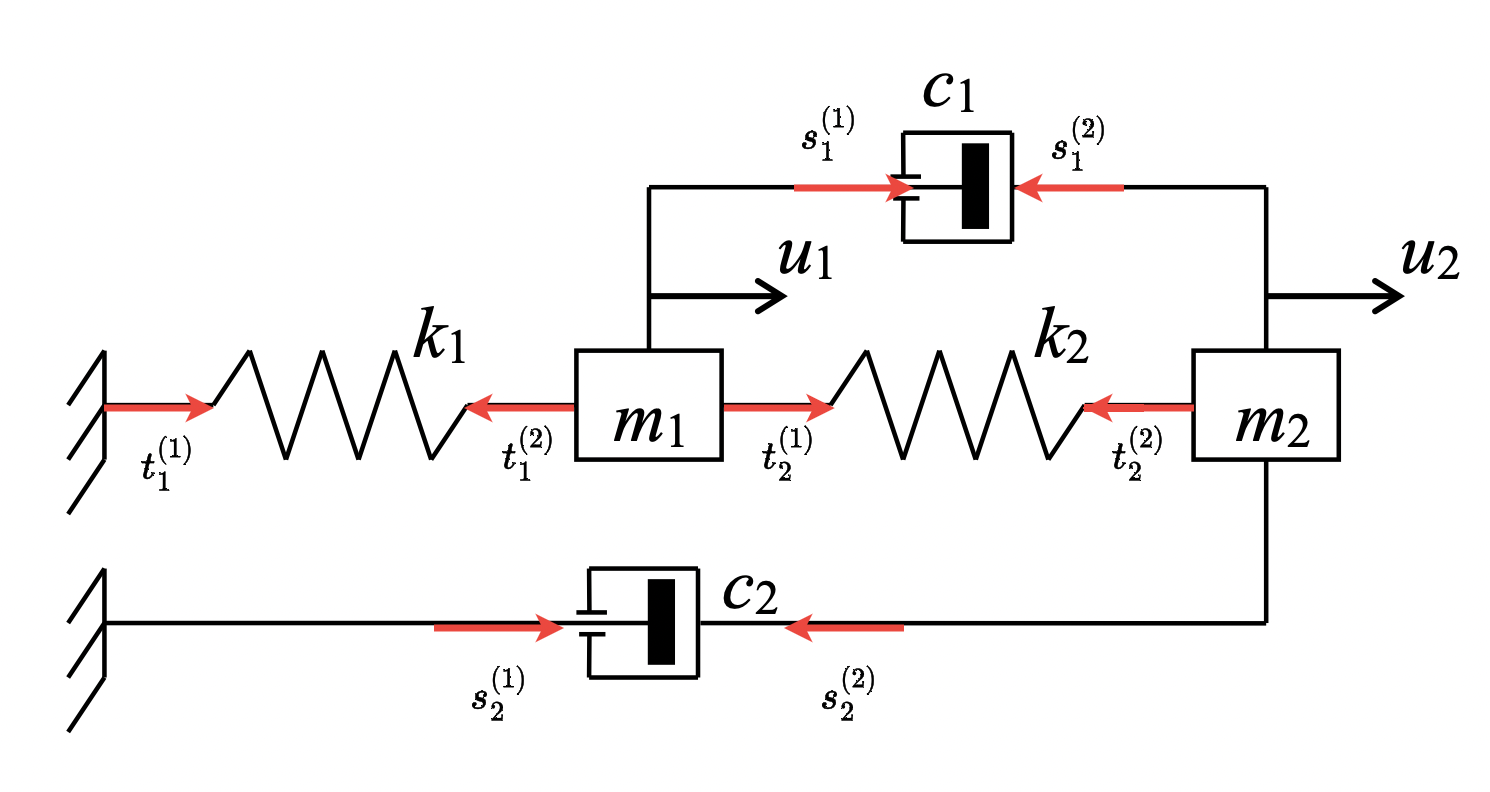
\includegraphics[width=1\textwidth]{task1.png}

Составим уравнения:
\[\begin{cases}
m_1\ddot u_1 + t_1^{(2)} + t_2^{(1)} + s_1^{(1)} = 0 \\
m_2\ddot u_2 + t_2^{(2)} + s_2^{(2)} + s_1^{(2)} = 0
\end{cases}\]

\[\begin{cases}
t_1^{(2)} = k_1 u_1\\
t_2^{(1)} = k_2 (u_2 - u_1)\\
t_2^{(2)} = 
\end{cases}\]





































\end{document}